\chapter{计数器变式题（20题完整解析）}

% ============================================================
\section{题1：模7计数器}

\textbf{题目}：设计模7计数器（0→1→...→6→0→...），写VHDL和Testbench。

\begin{solution}[完整解答]

\textbf{【分析】}
$N=7$，位宽 $k=\lceil\log_2 7\rceil=3$。清零条件：$cnt = 6(110)$。

\textbf{【状态图】}
\begin{center}
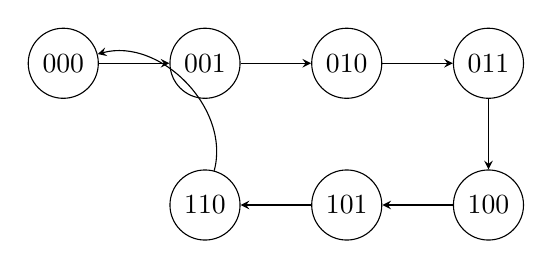
\begin{tikzpicture}[->,>=stealth,node distance=1.8cm]
\node[draw,circle] (s0) {000}; \node[draw,circle,right of=s0] (s1) {001};
\node[draw,circle,right of=s1] (s2) {010}; \node[draw,circle,right of=s2] (s3) {011};
\node[draw,circle,below of=s3] (s4) {100}; \node[draw,circle,left of=s4] (s5) {101};
\node[draw,circle,left of=s5] (s6) {110};
\draw (s0)--(s1); \draw (s1)--(s2); \draw (s2)--(s3);
\draw (s3)--(s4); \draw (s4)--(s5); \draw (s5)--(s6);
\draw (s6) edge[bend right=60] (s0);
\end{tikzpicture}
\end{center}

\textbf{【状态转移表】}
\begin{center}
\begin{tabular}{|c|c|c|}
\hline 当前状态(十进制) & 当前状态(二进制) & 下一状态 \\
\hline 0 & 000 & 001 \\ \hline 1 & 001 & 010 \\
\hline 2 & 010 & 011 \\ \hline 3 & 011 & 100 \\
\hline 4 & 100 & 101 \\ \hline 5 & 101 & 110 \\
\hline 6 & 110 & \textbf{000}（清零）\\
\hline
\end{tabular}
\end{center}

\textbf{【VHDL】}
\begin{lstlisting}
library ieee;
use ieee.std_logic_1164.all;
use ieee.std_logic_unsigned.all;

entity counter_mod7 is
  port (clk, rst_n : in std_logic;
        count : out std_logic_vector(2 downto 0);
        carry : out std_logic);
end counter_mod7;

architecture behavioral of counter_mod7 is
  signal cnt : std_logic_vector(2 downto 0);
begin
  process(clk, rst_n)
  begin
    if rst_n = '0' then
      cnt <= "000";
    elsif rising_edge(clk) then
      if cnt = "110" then     -- =6
        cnt <= "000";
      else
        cnt <= cnt + 1;
      end if;
    end if;
  end process;
  count <= cnt;
  carry <= '1' when cnt = "110" else '0';
end behavioral;
\end{lstlisting}

\textbf{【Testbench】}
\begin{lstlisting}
entity counter_mod7_tb is end entity;
architecture test of counter_mod7_tb is
  signal clk, rst_n, carry : std_logic;
  signal count : std_logic_vector(2 downto 0);
  constant T : time := 20 ns;
begin
  uut: entity work.counter_mod7 port map(clk, rst_n, count, carry);
  clk <= not clk after T/2;
  process begin
    rst_n <= '0'; wait for 30 ns;
    rst_n <= '1';
    -- 观察两个完整循环(14拍)
    wait for 14*T;
    wait;
  end process;
end test;
\end{lstlisting}

\textbf{【波形分析】}
\begin{center}
\begin{tabular}{|c|c|c|}
\hline 时钟拍 & count(二进制) & 十进制 \\ \hline
1 & 001 & 1 \\ \hline
2 & 010 & 2 \\ \hline
...&...&...\\ \hline
6 & 110 & 6 \\ \hline
7 & 000 & 0（carry=1！）\\ \hline
8 & 001 & 1（新循环）\\ \hline
\end{tabular}
\end{center}
验证：第7拍count归零且carry=1，第8拍count=1，循环正确。

\end{solution}

\begin{quickkill}
$k=\lceil\log_2 N\rceil$，清零条件=$N{-}1$。套模板：\texttt{if cnt = N-1 then cnt<=0; else cnt<=cnt+1;}
\end{quickkill}


% ============================================================
\section{题2：模5计数器}

\textbf{题目}：设计模5计数器（0→1→2→3→4→0→...），写出完整VHDL。

\begin{solution}[完整解答]

\textbf{【分析】}$N=5$，$k=\lceil\log_2 5\rceil=3$位。清零条件：$cnt=4(100)$。

\textbf{【状态序列】}$000 \to 001 \to 010 \to 011 \to 100 \to 000$

\textbf{【VHDL】}
\begin{lstlisting}
library ieee;
use ieee.std_logic_1164.all;
use ieee.std_logic_unsigned.all;

entity counter_mod5 is
  port (clk, rst_n : in std_logic;
        count : out std_logic_vector(2 downto 0);
        carry : out std_logic);
end counter_mod5;

architecture behavioral of counter_mod5 is
  signal cnt : std_logic_vector(2 downto 0);
begin
  process(clk, rst_n)
  begin
    if rst_n = '0' then cnt <= "000";
    elsif rising_edge(clk) then
      if cnt = "100" then cnt <= "000";  -- =4清零
      else cnt <= cnt + 1;
      end if;
    end if;
  end process;
  count <= cnt;
  carry <= '1' when cnt = "100" else '0';
end behavioral;
\end{lstlisting}

\textbf{【验证】}5拍一个循环。第5拍cnt=100(4)且carry=1，下一拍归零。

\textbf{【注意】}状态101/110/111（5-7）永远不会出现——这是正常现象，3位能表示0-7但只用了0-4。

\end{solution}


% ============================================================
\section{题3：模12计数器}

\textbf{题目}：设计模12计数器（0→1→...→11→0），并解释为什么不能自然溢出。

\begin{solution}[完整解答]

\textbf{【分析】}$N=12$，$k=\lceil\log_2 12\rceil=4$位。清零条件：$cnt=11(1011)$。

\textbf{【为什么不能自然溢出】}4位自然溢出=模16。如果不加清零逻辑，1111+1=0000，会经过16个状态而不是12个。必须显式在cnt=11时清零。

\textbf{【VHDL】}
\begin{lstlisting}
library ieee;
use ieee.std_logic_1164.all;
use ieee.std_logic_unsigned.all;

entity counter_mod12 is
  port (clk, rst_n : in std_logic;
        count : out std_logic_vector(3 downto 0);
        carry : out std_logic);
end counter_mod12;

architecture behavioral of counter_mod12 is
  signal cnt : std_logic_vector(3 downto 0);
begin
  process(clk, rst_n)
  begin
    if rst_n = '0' then cnt <= "0000";
    elsif rising_edge(clk) then
      if cnt = "1011" then cnt <= "0000";  -- =11清零
      else cnt <= cnt + 1;
      end if;
    end if;
  end process;
  count <= cnt;
  carry <= '1' when cnt = "1011" else '0';
end behavioral;
\end{lstlisting}

\textbf{【Testbench关键验证点】}
\begin{itemize}
  \item 第12拍：cnt=1011(11)，carry=1
  \item 第13拍：cnt=0000(0)（归零！）
  \item 第14拍：cnt=0001(1)（新循环开始）
\end{itemize}

\end{solution}


% ============================================================
\section{题4：模13计数器}

\textbf{题目}：设计模13计数器（0→1→...→12→0）。

\begin{solution}[完整解答]

\textbf{【分析】}$N=13$，$k=\lceil\log_2 13\rceil=4$位。清零条件：$cnt=12(1100)$。

\textbf{【VHDL】}
\begin{lstlisting}
signal cnt : std_logic_vector(3 downto 0);
-- 清零条件：cnt = "1100"  (=12)
 if cnt = "1100" then cnt <= "0000";
else cnt <= cnt + 1; end if;
\end{lstlisting}

\textbf{【完整状态序列】}
$$0000\to0001\to0010\to0011\to0100\to0101\to0110\to0111$$
$$\to1000\to1001\to1010\to1011\to1100\to0000$$

共13个状态。状态1101/1110/1111（13-15）永不出现。

\end{solution}


% ============================================================
\section{题5：模24计数器}

\textbf{题目}：设计模24计数器（0→1→...→23→0），用于小时计数器。

\begin{solution}[完整解答]

\textbf{【分析】}$N=24$，$k=\lceil\log_2 24\rceil=5$位。清零条件：$cnt=23(10111)$。

\textbf{【VHDL】}
\begin{lstlisting}
library ieee;
use ieee.std_logic_1164.all;
use ieee.std_logic_unsigned.all;

entity counter_mod24 is
  port (clk, rst_n : in std_logic;
        count : out std_logic_vector(4 downto 0);
        carry : out std_logic);
end counter_mod24;

architecture behavioral of counter_mod24 is
  signal cnt : std_logic_vector(4 downto 0);
begin
  process(clk, rst_n)
  begin
    if rst_n = '0' then cnt <= (others => '0');
    elsif rising_edge(clk) then
      if cnt = "10111" then cnt <= (others => '0');
      else cnt <= cnt + 1;
      end if;
    end if;
  end process;
  count <= cnt;
  carry <= '1' when cnt = "10111" else '0';
end behavioral;
\end{lstlisting}

\textbf{【状态范围】}00000(0)→00001(1)→...→10111(23)→00000(0)

注意：5位最多表示31，剩余8个状态(11000-11111)永不出现。

\textbf{【应用】}数字钟的小时计数器。

\end{solution}


% ============================================================
\section{题6：模60计数器（二进制）}

\textbf{题目}：设计模60计数器（0→1→...→59→0），用于秒/分计数器。

\begin{solution}[完整解答]

\textbf{【分析】}$N=60$，$k=\lceil\log_2 60\rceil=6$位。清零条件：$cnt=59(111011)$。

\textbf{【VHDL】}
\begin{lstlisting}
library ieee;
use ieee.std_logic_1164.all;
use ieee.std_logic_unsigned.all;

entity counter_mod60 is
  port (clk, rst_n : in std_logic;
        count : out std_logic_vector(5 downto 0);
        carry : out std_logic);
end counter_mod60;

architecture behavioral of counter_mod60 is
  signal cnt : std_logic_vector(5 downto 0);
begin
  process(clk, rst_n)
  begin
    if rst_n = '0' then cnt <= (others => '0');
    elsif rising_edge(clk) then
      if cnt = "111011" then cnt <= (others => '0');
      else cnt <= cnt + 1;
      end if;
    end if;
  end process;
  count <= cnt;
  carry <= '1' when cnt = "111011" else '0';
end behavioral;
\end{lstlisting}

\textbf{【二进制 vs BCD模60】}
\begin{itemize}
  \item 二进制模60：一个6位整体计数器（如本题）
  \item BCD模60：十位(模6)+个位(模10)级联
  \item 考试中要注意区分"二进制模60"和"BCD模60"
\end{itemize}

\end{solution}


% ============================================================
\section{题7：模10 BCD计数器}

\textbf{题目}：设计模10 BCD计数器（0→1→...→9→0）。个位，4位输出，BCD编码。

\begin{solution}[完整解答]

\textbf{【分析】}$N=10$，$k=4$位。状态：0000→0001→...→1001→0000。状态1010-1111不允许出现。

\textbf{【VHDL】}
\begin{lstlisting}
library ieee;
use ieee.std_logic_1164.all;
use ieee.std_logic_unsigned.all;

entity bcd_counter_mod10 is
  port (clk, rst_n : in std_logic;
        bcd : out std_logic_vector(3 downto 0);
        carry : out std_logic);
end bcd_counter_mod10;

architecture behavioral of bcd_counter_mod10 is
  signal cnt : std_logic_vector(3 downto 0);
begin
  process(clk, rst_n)
  begin
    if rst_n = '0' then cnt <= "0000";
    elsif rising_edge(clk) then
      if cnt = "1001" then cnt <= "0000";  -- =9清零
      else cnt <= cnt + 1;
      end if;
    end if;
  end process;
  bcd <= cnt;
  carry <= '1' when cnt = "1001" else '0';
end behavioral;
\end{lstlisting}

\textbf{【关键】}与普通模10计数器的区别：BCD的每个十进制位是独立4位，显示友好。

\end{solution}


% ============================================================
\section{题8：模60 BCD计数器（级联方案）}

\textbf{题目}：设计BCD模60计数器，个位(模10)+十位(模6)。输出十位和个位各4位BCD码。

\begin{solution}[完整解答]

\textbf{【分析】}
个位：模10，满9→清零并向十位进位。
十位：收到进位+1，十位模6（0-5）。
整体清零条件：十位=5且个位=9（即59）。

\textbf{【VHDL】}
\begin{lstlisting}
library ieee;
use ieee.std_logic_1164.all;
use ieee.std_logic_unsigned.all;

entity bcd_mod60 is
  port (clk, rst_n : in std_logic;
        tens, units : out std_logic_vector(3 downto 0));
end bcd_mod60;

architecture behavioral of bcd_mod60 is
  signal u_cnt : std_logic_vector(3 downto 0);  -- 个位
  signal t_cnt : std_logic_vector(3 downto 0);  -- 十位
begin
  process(clk, rst_n)
  begin
    if rst_n = '0' then
      u_cnt <= "0000"; t_cnt <= "0000";
    elsif rising_edge(clk) then
      -- 整体清零：59→00
      if t_cnt = "0101" and u_cnt = "1001" then
        u_cnt <= "0000"; t_cnt <= "0000";
      -- 个位满9→进位
      elsif u_cnt = "1001" then
        u_cnt <= "0000";
        t_cnt <= t_cnt + 1;
      else
        u_cnt <= u_cnt + 1;
      end if;
    end if;
  end process;
  tens <= t_cnt; units <= u_cnt;
end behavioral;
\end{lstlisting}

\textbf{【状态演化（关键节点）】}
\begin{center}
\begin{tabular}{|c|c|c|}
\hline 拍 & 十位(tens) & 个位(units) \\ \hline
9 & 0000 & 1001 \\ \hline
10 & 0001 & 0000（个位进位！）\\ \hline
19 & 0001 & 1001 \\ \hline
20 & 0010 & 0000 \\ \hline
...&...&...\\ \hline
59 & 0101 & 1001 \\ \hline
60 & 0000 & 0000（整体清零！）\\ \hline
\end{tabular}
\end{center}

\textbf{【验证要点】}
第10拍：个位从9变0，十位从0变1——进位正确。
第60拍：59→00——整体清零正确。

\end{solution}


% ============================================================
\section{题9：模24 BCD计数器（级联方案）}

\textbf{题目}：设计BCD模24计数器。十位模3（0-2），个位模10（0-9）。整体清零条件：23。

\begin{solution}[完整解答]

\textbf{【VHDL】}
\begin{lstlisting}
entity bcd_mod24 is
  port (clk, rst_n : in std_logic;
        tens, units : out std_logic_vector(3 downto 0));
end bcd_mod24;

architecture behavioral of bcd_mod24 is
  signal u_cnt, t_cnt : std_logic_vector(3 downto 0);
begin
  process(clk, rst_n)
  begin
    if rst_n = '0' then
      u_cnt <= "0000"; t_cnt <= "0000";
    elsif rising_edge(clk) then
      -- 整体清零：23→00
      if t_cnt = "0010" and u_cnt = "0011" then
        u_cnt <= "0000"; t_cnt <= "0000";
      elsif u_cnt = "1001" then
        u_cnt <= "0000";
        t_cnt <= t_cnt + 1;
      else
        u_cnt <= u_cnt + 1;
      end if;
    end if;
  end process;
  tens <= t_cnt; units <= u_cnt;
end behavioral;
\end{lstlisting}

\textbf{【注意】}十位的模3约束由清零条件隐式保证——计到23就清零，所以十位永远不会达到3。

\end{solution}


% ============================================================
\section{题10：模100 BCD计数器}

\textbf{题目}：设计BCD模100计数器（00→01→...→99→00）。

\begin{solution}[完整解答]

\textbf{【分析】}个位模10，十位模10。清零条件：十位=9且个位=9（即99）。

\textbf{【VHDL】}
\begin{lstlisting}
entity bcd_mod100 is
  port (clk, rst_n : in std_logic;
        tens, units : out std_logic_vector(3 downto 0));
end bcd_mod100;

architecture behavioral of bcd_mod100 is
  signal u_cnt, t_cnt : std_logic_vector(3 downto 0);
begin
  process(clk, rst_n)
  begin
    if rst_n = '0' then
      u_cnt <= "0000"; t_cnt <= "0000";
    elsif rising_edge(clk) then
      if t_cnt = "1001" and u_cnt = "1001" then  -- 99
        u_cnt <= "0000"; t_cnt <= "0000";
      elsif u_cnt = "1001" then
        u_cnt <= "0000";
        t_cnt <= t_cnt + 1;
      else
        u_cnt <= u_cnt + 1;
      end if;
    end if;
  end process;
  tens <= t_cnt; units <= u_cnt;
end behavioral;
\end{lstlisting}

\end{solution}


% ============================================================
\section{题11：带使能端en的模8计数器}

\textbf{题目}：设计带使能信号的模8计数器。en=1计数，en=0保持当前值。

\begin{solution}[完整解答]

\textbf{【分析】}模8=$2^3$，自然溢出即可。增加en控制是否+1。

\textbf{【VHDL】}
\begin{lstlisting}
entity counter_mod8_en is
  port (clk, rst_n, en : in std_logic;
        count : out std_logic_vector(2 downto 0));
end counter_mod8_en;

architecture behavioral of counter_mod8_en is
  signal cnt : std_logic_vector(2 downto 0);
begin
  process(clk, rst_n)
  begin
    if rst_n = '0' then cnt <= "000";
    elsif rising_edge(clk) then
      if en = '1' then
        cnt <= cnt + 1;  -- 3位自然溢出=模8
      end if;
      -- en='0': 不赋值 → 保持
    end if;
  end process;
  count <= cnt;
end behavioral;
\end{lstlisting}

\textbf{【Testbench关键测试】}
\begin{itemize}
  \item en=1时正常计数（0,1,2,...→7→0）
  \item en=0时count保持不变
  \item en从0切换为1时从当前值继续计数
\end{itemize}

\end{solution}


% ============================================================
\section{题12：带同步加载的模10计数器}

\textbf{题目}：设计带load端口的模10计数器。load=1时cnt=data\_in；load=0时正常计数(0-9)。

\begin{solution}[完整解答]

\textbf{【VHDL】}
\begin{lstlisting}
entity counter_mod10_load is
  port (clk, rst_n, load : in std_logic;
        data_in : in std_logic_vector(3 downto 0);
        count : out std_logic_vector(3 downto 0));
end counter_mod10_load;

architecture behavioral of counter_mod10_load is
  signal cnt : std_logic_vector(3 downto 0);
begin
  process(clk, rst_n)
  begin
    if rst_n = '0' then cnt <= "0000";
    elsif rising_edge(clk) then
      if load = '1' then
        cnt <= data_in;           -- 同步加载
      elsif cnt = "1001" then
        cnt <= "0000";            -- 满9清零
      else
        cnt <= cnt + 1;
      end if;
    end if;
  end process;
  count <= cnt;
end behavioral;
\end{lstlisting}

\textbf{【注意】}load优先级高于计数。if-else顺序决定优先级——if在最前面优先级最高。

\end{solution}


% ============================================================
\section{题13：双向计数器（递增/递减）}

\textbf{题目}：设计模16双向计数器。up=1递增，up=0递减。

\begin{solution}[完整解答]

\textbf{【VHDL】}
\begin{lstlisting}
entity counter_updown is
  port (clk, rst_n, up : in std_logic;
        count : out std_logic_vector(3 downto 0));
end counter_updown;

architecture behavioral of counter_updown is
  signal cnt : std_logic_vector(3 downto 0);
begin
  process(clk, rst_n)
  begin
    if rst_n = '0' then cnt <= "0000";
    elsif rising_edge(clk) then
      if up = '1' then
        cnt <= cnt + 1;  -- 递增
      else
        cnt <= cnt - 1;  -- 递减
      end if;
    end if;
  end process;
  count <= cnt;
end behavioral;
\end{lstlisting}

\textbf{【递减行为】}cnt-1：当cnt=0000时，0000-1 = 1111（二进制借位），所以是模16递减计数器。

\textbf{【状态序列（递减）】}$0000 \to 1111 \to 1110 \to \dots \to 0001 \to 0000$

\end{solution}


% ============================================================
\section{题14：多个计数器级联——模40}

\textbf{题目}：模8计数器 + 模5计数器级联。总模值？写出联逻辑。

\begin{solution}[完整解答]

\textbf{【分析】}总模值=$M_1 \times M_2 = 8 \times 5 = 40$。

\textbf{【级联逻辑】}
模8计数器每8拍carry=1一次。模5计数器以carry作为使能，收到carry=1时+1。

\textbf{【VHDL】}
\begin{lstlisting}
entity counter_mod40_cascade is
  port (clk, rst_n : in std_logic;
        count_lo : out std_logic_vector(2 downto 0);  -- 模8
        count_hi : out std_logic_vector(2 downto 0)); -- 模5
end counter_mod40_cascade;

architecture behavioral of counter_mod40_cascade is
  signal cnt8 : std_logic_vector(2 downto 0);
  signal cnt5 : std_logic_vector(2 downto 0);
  signal carry8 : std_logic;
begin
  -- 模8（低位）
  process(clk, rst_n)
  begin
    if rst_n = '0' then cnt8 <= "000";
    elsif rising_edge(clk) then
      cnt8 <= cnt8 + 1;  -- 3位自然溢出=模8
    end if;
  end process;
  carry8 <= '1' when cnt8 = "111" else '0';

  -- 模5（高位）
  process(clk, rst_n)
  begin
    if rst_n = '0' then cnt5 <= "000";
    elsif rising_edge(clk) then
      if carry8 = '1' then
        if cnt5 = "100" then cnt5 <= "000";  -- =4清零
        else cnt5 <= cnt5 + 1;
        end if;
      end if;
    end if;
  end process;

  count_lo <= cnt8; count_hi <= cnt5;
end behavioral;
\end{lstlisting}

\textbf{【通用公式】}级联总模值 = $M_1 \times M_2 \times \cdots \times M_k$

\end{solution}


% ============================================================
\section{题15：给定VHDL推断模值}

\textbf{题目}：分析以下代码，推断计数器的模值N。
\begin{lstlisting}
 if cnt = "1010" then cnt <= "0000";
else cnt <= cnt + 1; end if;
\end{lstlisting}

\begin{solution}[完整解答]

\textbf{【分析】}清零条件：cnt=1010=10。

\textbf{【关键公式】}模值 = 清零比较值 + 1

当cnt=10时清零，意味着cnt经过了状态0,1,2,...,10，共11个状态后被清零。

所以N=10+1=11。

\textbf{【验证】}
状态序列：0→1→2→3→4→5→6→7→8→9→10→0
共11个不同的状态（0到10），模值=11。

\textbf{【常见陷阱】}不能只看清零值！清零值=10但模值=11。因为cnt=10这一个状态本身也算一个状态。

\textbf{【万能公式】}$N = (\text{清零比较的数值}) + 1$

\end{solution}

\begin{quickkill}
\textbf{模值 = 清零条件中的比较值 + 1}

cnt = X 时清零 → 模值 = X + 1
\end{quickkill}


% ============================================================
\section{题16：带暂停的模12计数器}

\textbf{题目}：设计带暂停信号pause的模12计数器。pause=1暂停，pause=0恢复。

\begin{solution}[完整解答]

\textbf{【VHDL】}
\begin{lstlisting}
entity counter_mod12_pause is
  port (clk, rst_n, pause : in std_logic;
        count : out std_logic_vector(3 downto 0));
end counter_mod12_pause;

architecture behavioral of counter_mod12_pause is
  signal cnt : std_logic_vector(3 downto 0);
begin
  process(clk, rst_n)
  begin
    if rst_n = '0' then cnt <= "0000";
    elsif rising_edge(clk) then
      if pause = '0' then
        if cnt = "1011" then cnt <= "0000";
        else cnt <= cnt + 1;
        end if;
      end if;
      -- pause='1': 不赋值 → 保持
    end if;
  end process;
  count <= cnt;
end behavioral;
\end{lstlisting}

\textbf{【Testbench关键验证】}
\begin{itemize}
  \item pause=0：正常0→1→...→11→0
  \item pause=1：cnt保持不变
  \item pause从1→0：从保持的值继续计数
\end{itemize}

\end{solution}


% ============================================================
\section{题17：倒计时计数器（递减，预置值→0）}

\textbf{题目}：设计从预置值PRE递减到0的倒计时计数器。到0后重新加载PRE。

\begin{solution}[完整解答]

\textbf{【VHDL】}
\begin{lstlisting}
entity down_counter is
  generic (PRE : integer := 9);
  port (clk, rst_n : in std_logic;
        count : out std_logic_vector(3 downto 0);
        zero : out std_logic);
end down_counter;

architecture behavioral of down_counter is
  signal cnt : std_logic_vector(3 downto 0);
begin
  process(clk, rst_n)
  begin
    if rst_n = '0' then
      cnt <= std_logic_vector(to_unsigned(PRE, 4));
    elsif rising_edge(clk) then
      if cnt = "0000" then
        cnt <= std_logic_vector(to_unsigned(PRE, 4));
      else
        cnt <= cnt - 1;
      end if;
    end if;
  end process;
  count <= cnt;
  zero <= '1' when cnt = "0000" else '0';
end behavioral;
\end{lstlisting}

\textbf{【状态序列(PRE=9)】}$9\to8\to7\to6\to5\to4\to3\to2\to1\to0\to9\to8\to\cdots$

\end{solution}


% ============================================================
\section{题18：数字钟核心——时/分/秒级联}

\textbf{题目}：设计时(H):分(M):秒(S)三层级联BCD计数器。S和M为模60，H为模24。

\begin{solution}[完整解答]

\textbf{【架构】}
\begin{center}
\begin{tikzpicture}[->,>=stealth]
\node[draw,minimum width=2cm,minimum height=1cm] (s) at (0,0) {模60（秒）};
\node[draw,minimum width=2cm,minimum height=1cm] (m) at (3.5,0) {模60（分）};
\node[draw,minimum width=2cm,minimum height=1cm] (h) at (7,0) {模24（时）};
\draw (s.east)--(m.west) node[midway,above]{carry};
\draw (m.east)--(h.west) node[midway,above]{carry};
\end{tikzpicture}
\end{center}
秒满60→分+1，分满60→时+1，时满24→时归零。

\textbf{【VHDL】}
\begin{lstlisting}
entity digital_clock is
  port (clk, rst_n : in std_logic;
        sec_u, sec_t : out std_logic_vector(3 downto 0);
        min_u, min_t : out std_logic_vector(3 downto 0);
        hour_u, hour_t : out std_logic_vector(3 downto 0));
end digital_clock;

architecture behavioral of digital_clock is
  signal s_u, s_t, m_u, m_t, h_u, h_t : std_logic_vector(3 downto 0);
  signal s_carry, m_carry : std_logic;
begin
  process(clk, rst_n)
  begin
    if rst_n = '0' then
      s_u <= x"0"; s_t <= x"0"; m_u <= x"0"; m_t <= x"0";
      h_u <= x"0"; h_t <= x"0"; s_carry <= '0'; m_carry <= '0';
    elsif rising_edge(clk) then
      s_carry <= '0'; m_carry <= '0';

      -- 秒个位计数
      if s_u = x"9" then s_u <= x"0";
        if s_t = x"5" then
          s_t <= x"0"; s_carry <= '1';  -- 59→00秒, 进位到分
        else s_t <= s_t + 1;
        end if;
      else s_u <= s_u + 1;
      end if;

      -- 分计数（收到秒进位时）
      if s_carry = '1' then
        if m_u = x"9" then m_u <= x"0";
          if m_t = x"5" then
            m_t <= x"0"; m_carry <= '1';  -- 59→00分, 进位到时
          else m_t <= m_t + 1;
          end if;
        else m_u <= m_u + 1;
        end if;
      end if;

      -- 时计数（收到分进位时）
      if m_carry = '1' then
        if h_t = x"2" and h_u = x"3" then  -- 23→00
          h_t <= x"0"; h_u <= x"0";
        elsif h_u = x"9" then
          h_u <= x"0"; h_t <= h_t + 1;
        else h_u <= h_u + 1;
        end if;
      end if;
    end if;
  end process;

  sec_u <= s_u; sec_t <= s_t;
  min_u <= m_u; min_t <= m_t;
  hour_u <= h_u; hour_t <= h_t;
end behavioral;
\end{lstlisting}

\end{solution}


% ============================================================
\section{题19：计数器最大工作频率分析}

\textbf{题目}：4位行波进位计数器，D触发器$t_{cko}=2$ns，$t_{setup}=1$ns，每级进位延迟3ns。求$f_{max}$。

\begin{solution}[完整解答]

\textbf{【关键路径】}
从D触发器输出→加法器进位链（4级×3ns=12ns）→下一个D触发器setup时间

$$t_{critical} = t_{cko} + 4 \times t_{carry} + t_{setup}$$
$$= 2 + 12 + 1 = 15\text{ns}$$

$$f_{max} = \frac{1}{15\text{ns}} = 66.7\text{MHz}$$

\textbf{【如果改用超前进位】}
进位延迟从$O(N)$降为$O(1)$，$f_{max}$可大幅提升。

\textbf{【考试公式】}$f_{max} = 1 / (t_{cko} + N \times t_{carry} + t_{setup})$

N=计数器位数，$t_{carry}$=每级进位延迟。

\end{solution}


% ============================================================
\section{题20：格雷码计数器}

\textbf{题目}：设计3位格雷码计数器（000→001→011→010→110→111→101→100→000...）。

\begin{solution}[完整解答]

\textbf{【分析】}格雷码：相邻状态只有1位不同。3位格雷码共8个状态（模8）。

\textbf{【格雷码序列（3位）】}
\begin{center}
\begin{tabular}{|c|c|c|}
\hline 状态编号 & 格雷码 & 下一状态格雷码 \\ \hline
0 & 000 & 001 \\ \hline 1 & 001 & 011 \\ \hline
2 & 011 & 010 \\ \hline 3 & 010 & 110 \\ \hline
4 & 110 & 111 \\ \hline 5 & 111 & 101 \\ \hline
6 & 101 & 100 \\ \hline 7 & 100 & 000 \\ \hline
\end{tabular}
\end{center}

\textbf{【VHDL——直接case实现】}
\begin{lstlisting}
entity gray_counter_3bit is
  port (clk, rst_n : in std_logic;
        gray : out std_logic_vector(2 downto 0));
end gray_counter_3bit;

architecture behavioral of gray_counter_3bit is
  signal g : std_logic_vector(2 downto 0);
begin
  process(clk, rst_n)
  begin
    if rst_n = '0' then g <= "000";
    elsif rising_edge(clk) then
      case g is
        when "000" => g <= "001";
        when "001" => g <= "011";
        when "011" => g <= "010";
        when "010" => g <= "110";
        when "110" => g <= "111";
        when "111" => g <= "101";
        when "101" => g <= "100";
        when "100" => g <= "000";
        when others => g <= "000";
      end case;
    end if;
  end process;
  gray <= g;
end behavioral;
\end{lstlisting}

\textbf{【应用】}格雷码计数器常用于FIFO的读写指针——相邻状态只变1位，减少亚稳态风险。

\end{solution}


% ============================================================
\section{计数器类题目：统一秒杀总结}

\begin{quickkill}[计数器20题秒杀总结]
\textbf{步骤1：}确定模值N，位宽$k=\lceil\log_2 N\rceil$

\textbf{步骤2：}清零条件 = N-1（二进制）

\textbf{步骤3：}套用统一模板：
\begin{lstlisting}
 if cnt = (N-1) then cnt <= 0; else cnt <= cnt + 1; end if;
\end{lstlisting}

\textbf{步骤4：}如有额外控制（en, load, pause, up/down），用if-else设定优先级

\textbf{步骤5：}BCD级联：低位carry接高位使能，整体清零条件同时清零多级

\textbf{关键公式：}
\begin{itemize}
  \item 模值 = 清零比较值 + 1
  \item 级联总模值 = $M_1 \times M_2 \times \cdots$
  \item $2^N$模值（如模16、模8）：不需要显式清零（自然溢出）
  \item $f_{max} = 1/(t_{cko} + N{\times}t_{carry} + t_{setup})$
\end{itemize}

\textbf{所有计数器题目的答案都是同一个模板改参数。}
\end{quickkill}
